\begin{figure}[htbp]
    \centering
    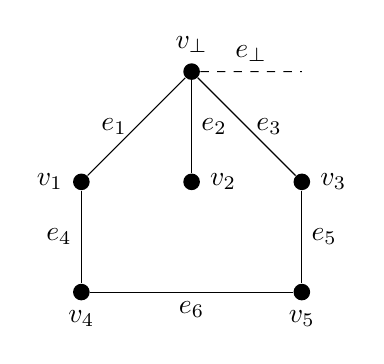
\begin{tikzpicture}[scale=0.7]
        % Vertices
        \node (v0) at (0, 3) [circle, fill, inner sep=1pt, minimum size=6pt, label=above:$v_\bot$] {};
        \node (v1) at (-2, 1) [circle, fill, inner sep=1pt, minimum size=6pt, label=left:$v_1$] {};
        \node (v2) at (0, 1) [circle, fill, inner sep=1pt, minimum size=6pt, label=right:$v_2$] {};
        \node (v3) at (2, 1) [circle, fill, inner sep=1pt, minimum size=6pt, label=right:$v_3$] {};
        \node (v4) at (-2, -1) [circle, fill, inner sep=1pt, minimum size=6pt, label=below:$v_4$] {};
        \node (v5) at (2, -1) [circle, fill, inner sep=1pt, minimum size=6pt, label=below:$v_5$] {};
        % Edges
        \draw[dashed] (v0) -- (2, 3) node[midway, above] {$e_{\bot}$};
        \draw (v0) -- (v1) node[midway, left] {$e_1$};
        \draw (v0) -- (v2) node[midway, right] {$e_2$};
        \draw (v0) -- (v3) node[midway, right] {$e_3$};
        \draw (v1) -- (v4) node[midway, left] {$e_4$};
        \draw (v3) -- (v5) node[midway, right] {$e_5$};
        \draw (v4) -- (v5) node[midway, below] {$e_6$};
    \end{tikzpicture}
    \caption{A counterexample against the arbitrary choice of edges. The unique half-edge is $e_\bot$ incident to $v_\bot$ and $\set{e_1, e_2, \ldots, e_6}$ are normal edges. The signatures are set as $f_{v_\bot} = [1, 1, 1, 0]$, $f_{v_2} = [1, 1]$ and $f_{v_1} = f_{v_3} = f_{v_4} = f_{v_5} = [1, 10]$. Consider two partial assignments $\sigma = (e_\bot \gets 1)$ and $\tau = (e_\bot \gets 0)$. Then it holds that $\Ham(\sigma, v_\bot) > \Ham(\tau, v_\bot)$ but $\mu_{e_2}^{\sigma}(1) = \frac{10301}{24622} > \frac{14321}{38742} = \mu_{e_2}^{\tau}(1)$.}
    \label{fig:edge-selection-counterexample}
\end{figure}